\documentclass[aspectratio=169]{beamer}
\usepackage{beamerthemeAMU}
\usepackage{amsmath}
\usepackage{booktabs}
\usepackage{array}
\usepackage{listings}
\usepackage{hyperref}
\usepackage{tikz}
\usetikzlibrary{arrows.meta,positioning,calc,matrix}

% TikZ styles for reusable LLM flow elements
\colorlet{llmInputBg}{AMU_acc5!35!AMU_lt1}
\colorlet{llmCoreBg}{AMU_dk2!15!AMU_lt1}
\colorlet{llmOutputBg}{AMU_lt2!70!AMU_lt1}
\colorlet{llmInputAccent}{AMU_acc6}
\colorlet{llmTextAccent}{AMU_dk2}
\colorlet{llmEmbedA}{AMU_acc5}
\colorlet{llmEmbedB}{AMU_dk2!60!AMU_lt1}
\colorlet{llmEmbedC}{AMU_acc6!70!AMU_lt1}
\colorlet{llmEmbedD}{AMU_acc1}
\colorlet{llmGray}{AMU_dk1!65!AMU_lt1}
\colorlet{llmGrayLight}{AMU_dk1!40!AMU_lt1}
\colorlet{llmArrow}{AMU_acc1}
\colorlet{llmCoreTitle}{AMU_dk2}

\colorlet{llmEmbedDroneA}{AMU_dk2!10}
\colorlet{llmEmbedDroneB}{AMU_dk2!30}
\colorlet{llmEmbedDroneC}{AMU_dk2!50}
\colorlet{llmEmbedDroneD}{AMU_dk2!70}
\colorlet{llmEmbedDroneE}{AMU_dk2!90}
\colorlet{llmEmbedSmartA}{AMU_acc6!10}
\colorlet{llmEmbedSmartB}{AMU_acc6!30}
\colorlet{llmEmbedSmartC}{AMU_acc6!50}
\colorlet{llmEmbedSmartD}{AMU_acc6!70}
\colorlet{llmEmbedSmartE}{AMU_acc6!90}



\colorlet{tokenSentenceBg}{AMU_dk2!12!AMU_lt1}
\colorlet{tokenSentenceBorder}{AMU_dk1!80!AMU_dk2}
\colorlet{tokenWordBgA}{AMU_acc5!70!AMU_lt1}
\colorlet{tokenWordBgB}{AMU_lt2!80!AMU_lt1}
\colorlet{tokenVocabBg}{AMU_lt2!60!AMU_lt1}
\colorlet{tokenConnector}{AMU_dk1!70!AMU_lt1}

\colorlet{neighborWordBg}{AMU_lt1}
\colorlet{neighborRedA}{AMU_acc3!30!AMU_lt1}
\colorlet{neighborRedB}{AMU_acc3!55!AMU_lt1}
\colorlet{neighborRedC}{AMU_acc3!75!AMU_lt1}
\colorlet{neighborRedD}{AMU_acc3!90!AMU_lt1}
\colorlet{neighborBlueA}{AMU_acc6!30!AMU_lt1}
\colorlet{neighborBlueB}{AMU_acc6!55!AMU_lt1}
\colorlet{neighborBlueC}{AMU_acc6!75!AMU_lt1}
\colorlet{neighborBlueD}{AMU_acc6!90!AMU_lt1}

\colorlet{dimCellGray}{AMU_dk1!25!AMU_lt1}
\colorlet{dimCellRed}{AMU_acc3!65!AMU_lt1}
\colorlet{dimCellBlue}{AMU_dk2!65!AMU_lt1}
\colorlet{dimCellOrange}{AMU_acc3!40!AMU_lt2}
\colorlet{dimCellPurple}{AMU_acc6!65!AMU_lt1}
\colorlet{dimCellGreen}{AMU_lt2!45!AMU_acc1}

\tikzset{llm/box/.style={draw=black, rounded corners=6pt, inner sep=10pt, align=center}}
\tikzset{llm/input/.style={llm/box, fill=llmInputBg, minimum width=6.8cm, minimum height=2.0cm}}
\tikzset{llm/core/.style={llm/box, fill=llmCoreBg, minimum width=6.2cm, minimum height=1.8cm}}
\tikzset{llm/outputEmbedding/.style={llm/box, fill=llmOutputBg, minimum width=3.8cm, minimum height=1.5cm}}
\tikzset{llm/output/.style={llm/box, fill=llmOutputBg, minimum width=3.8cm, minimum height=2.4cm}}
\tikzset{llm/arrow/.style={->, line width=1.2pt, >=Stealth, draw=llmArrow}}

\tikzset{token/sentenceLabel/.style={font=\bfseries\small, text=AMU_dk1}}
\tikzset{token/sentence/.style={draw=tokenSentenceBorder, fill=tokenSentenceBg, rounded corners=8pt, font=\small, inner xsep=12pt, inner ysep=8pt, align=center}}
\tikzset{token/arrow/.style={->, line width=1pt, >=Stealth, draw=tokenConnector}}
\tikzset{token/annotation/.style={font=\scriptsize, text=tokenConnector}}
\tikzset{token/word/.style={draw=AMU_dk1, rounded corners=6pt, font=\small\bfseries, inner xsep=10pt, inner ysep=7pt, align=center}}
\tikzset{token/wordA/.style={token/word, fill=tokenWordBgA}}
\tikzset{token/wordB/.style={token/word, fill=tokenWordBgB}}
\tikzset{token/bit/.style={token/word, fill=AMU_dk2!50}}
\tikzset{token/vocabWord/.style={token/word, fill=tokenVocabBg}}
\tikzset{token/vocabLabel/.style={font=\small\bfseries, text=AMU_dk1}}
\tikzset{token/span/.style={<->, line width=1pt, draw=tokenConnector, densely dashed}}

\tikzset{neighbor/colLabel/.style={font=\small\bfseries, text=AMU_dk1}}
\tikzset{neighbor/word/.style={draw=AMU_dk1, rounded corners=6pt, fill=neighborWordBg, inner xsep=10pt, inner ysep=6pt, font=\small}}
\tikzset{neighbor/embedCell/.style={draw=AMU_dk1!70!AMU_lt1, rounded corners=2pt, minimum width=0.58cm, minimum height=0.7cm}}
\tikzset{neighbor/arrow/.style={->, >=Stealth, line width=1pt, draw=tokenConnector}}
\tikzset{neighbor/nn/.style={draw=AMU_dk1, rounded corners=10pt, fill=tokenSentenceBg, inner xsep=16pt, inner ysep=14pt, align=left, font=\small}}
\tikzset{neighbor/prediction/.style={font=\bfseries\large, text=AMU_dk1}}
\tikzset{neighbor/predLabel/.style={font=\small\bfseries, text=llmGray}}

\tikzset{dim/wordHeading/.style={font=\small\bfseries, text=AMU_dk1}}
\tikzset{dim/rowLabel/.style={font=\small, text=llmGray, anchor=east}}
\tikzset{dim/cell/.style={draw=AMU_dk1, rounded corners=2pt, minimum width=1.2cm, minimum height=0.9cm, font=\small, inner sep=2pt}}
\tikzset{dim/cellGray/.style={dim/cell, fill=dimCellGray}}
\tikzset{dim/cellRed/.style={dim/cell, fill=dimCellRed}}
\tikzset{dim/cellBlue/.style={dim/cell, fill=dimCellBlue}}
\tikzset{dim/cellOrange/.style={dim/cell, fill=dimCellOrange}}
\tikzset{dim/cellPurple/.style={dim/cell, fill=dimCellPurple}}
\tikzset{dim/cellGreen/.style={dim/cell, fill=dimCellGreen}}
\tikzset{dim/dots/.style={font=\Large, text=llmGray}}
\tikzset{dim/axisArrow/.style={<->, densely dotted, line width=1pt, draw=tokenConnector}}
\tikzset{dim/axisLabel/.style={font=\small\bfseries, text=AMU_dk1}}
\tikzset{dim/axisLabelSub/.style={font=\footnotesize, text=llmGray}}

\newcommand{\llmParagraph}[4]{%
  \begin{scope}[shift={#1}]
    \foreach \offset/\length in {#3} {
      \draw[line width=#2, line cap=round, draw=#4] (0,\offset) -- ++(\length,0);
    }
  \end{scope}%
}

\newcommand{\llmEmbeddingBlocks}[3]{%
  \begin{scope}[shift={#1}]
    \foreach [count=\i] \shade in {#3} {
      \pgfmathsetmacro{\xshift}{(\i-1)*0.8}
      \path[draw=black, fill=\shade, rounded corners=2pt]
        (\xshift cm,-0.28cm) rectangle ++(0.65cm,0.65cm);
    }
  \end{scope}%
}

\newcommand{\llmEmbeddingBlocksSmall}[3]{%
  \begin{scope}[shift={#1}]
    \foreach [count=\i] \shade in {#3} {
      \pgfmathsetmacro{\xshift}{(\i-1)*0.6}
      \path[draw=black, fill=\shade, rounded corners=2pt]
        (\xshift cm,-0.18cm) rectangle ++(0.5cm,0.5cm);
    }
  \end{scope}%
}


\newcommand{\TokenWordRow}[4]{%
  \foreach [count=\i] \word in {#4} {
    \ifnum\i=1
      \node[#3] (#2-\i) at #1 {\strut \word};
    \else
      \pgfmathtruncatemacro{\prev}{\i-1}
      \node[#3, right=0.12cm of #2-\prev] (#2-\i) {\strut \word};
    \fi
  }%
}

\newcommand{\NeighborEmbeddingRow}[3]{%
  \foreach [count=\i] \shade in {#3} {
    \pgfmathsetmacro{\xshift}{(\i-1)*0.65}
    \node[neighbor/embedCell, fill=\shade] (#2-\i) at ($(#1)+(\xshift cm,0)$) {};
  }%
}



  



\newcommand{\LLMPipelineDiagram}{%
  \begin{tikzpicture}[font=\small, node distance=1.3cm and 2.2cm]
    \node[align=center, font=\bfseries] (inputlabel) {\large Text input\\{\normalsize\color{llmGray} Unstructured data}};
    \node[llm/input, below=0.4cm of inputlabel] (inputbox) {};

    \llmParagraph{($(inputbox.west)+(0.55cm,0)$)}{6pt}{0.45/4.8cm,0/4.5cm,-0.45/4.2cm}{llmInputAccent}

    \node[llm/core, below=1.5cm of inputbox] (core) {\textcolor{llmCoreTitle}{\bfseries Language AI}\\{\normalsize\color{llmGray} Processes the input text}};

    \draw[llm/arrow] (inputbox.south) -- (core.north);

    \coordinate (split) at ($(core.south)+(0,-0.6cm)$);
    \draw[llm/arrow] (core.south) -- (split);

    \node[llm/output, below left=2.9cm and 2.2cm of core] (textout) {};
    \node[llm/outputEmbedding, below=2.9cm of core] (embeddings) {};
    \node[llm/output, below right=2.9cm and 2.2cm of core] (classify) {};

    \node[align=center, font=\bfseries] at ($(textout.south)+(0,-1.0cm)$) {Text output\\{\normalsize\color{llmGray} Generative modeling}};
    \node[align=center, font=\bfseries] at ($(embeddings.south)+(0,-1.0cm)$) {Embeddings\\{\normalsize\color{llmGray} Numeric values}};
    \node[align=center, font=\bfseries] at ($(classify.south)+(0,-1.0cm)$) {Classification\\{\normalsize\color{llmGray} Identify targets}};

    \draw[llm/arrow] (split) -| (textout.north);
    \draw[llm/arrow] (split) -- (embeddings.north);
    \draw[llm/arrow] (split) -| (classify.north);

    \llmParagraph{($(textout.west)+(0.4cm,0.4cm)$)}{5pt}{0.3/2.2cm,-0.3/2.2cm,-0.9/2.2cm}{llmTextAccent}

    \llmEmbeddingBlocks{($(embeddings.west)+(0.35cm,0)$)}{black}{llmEmbedD, llmEmbedA,llmEmbedB,llmEmbedC}

    \llmParagraph{($(classify.west)+(0.4cm,0.4cm)$)}{5pt}{0/2.4cm}{llmTextAccent}
    \llmParagraph{($(classify.west)+(0.4cm,-0.12cm)$)}{5pt}{0/2.1cm,-0.6/2.2cm}{llmGrayLight}
  \end{tikzpicture}%
}

% Listing style for small code snippets
\lstset{basicstyle=\ttfamily\small,keywordstyle=\color{AMU_dk2}\bfseries,commentstyle=\itshape\color{gray},showstringspaces=false,columns=flexible}


\title{Large Language Models in Data Science}
\subtitle{Week 1: Concepts, Architecture, Motivation}
\author{Sebastian Mueller}
\institute{Aix-Marseille Universit\'e}
\date{2025-2026}

\begin{document}

\begin{frame}[plain]
  \titlepage
\end{frame}

\begin{frame}{Session Overview}
  \begin{columns}[T,onlytextwidth]
    \begin{column}{0.55\linewidth}
      \textbf{Lecture (1.5h)}
      \begin{enumerate}
        \item Why study LLMs now?
        \item From words to tokens
        \item Transformer architecture
        \item Training and inference
        \item Capabilities, limits, ecosystem
      \end{enumerate}
    \end{column}
    \begin{column}{0.4\linewidth}
      \textbf{Lab (1.5h)}
      \begin{itemize}
        \item Tokenize and embed real text
        \item Inspect different tokenizations and embeddings
      \end{itemize}
    \end{column}
  \end{columns}
\end{frame}

\section{Why Study LLMs?}

\begin{frame}{Motivation: Data Science is Changing}
  \begin{itemize}
    \item Analysts increasingly converse with their tools instead of writing boilerplate code.
    \item Reports, dashboards, and even experiments are drafted by generative models.
    \item Modern data workflows combine structured data with unstructured documents, code, and conversations.
    \item Understanding LLMs helps us design safer, more efficient assistants rather than treating them as black boxes.
  \end{itemize}
\end{frame}




\begin{frame}{What is a Large Language Model?}
  \begin{itemize}
    \item \textbf{Definition}: A neural network trained on massive text corpora to model the probability of token sequences.
    \item Given tokens $x_1, \dots, x_{t-1}$, the model estimates
      \[
        P(x_t \mid x_1, \dots, x_{t-1}).
      \]
    \item During inference the model samples one token at a time, feeding each prediction back as context.
    \item LLMs power question answering, summarization, code generation, and dialogue systems across industry.
  \end{itemize}
\end{frame}

\begin{frame}{LLM Capabilities}
  \centering
  \resizebox{!}{0.85\textheight}{\begin{tikzpicture}[font=\small, node distance=1.3cm and 2.2cm]
    \node[align=center, font=\bfseries] (inputlabel) {\large Text input\\{\normalsize\color{llmGray} Unstructured data}};
    \node[llm/input, below=0.4cm of inputlabel] (inputbox) {};

    \llmParagraph{($(inputbox.west)+(0.55cm,0)$)}{6pt}{0.45/4.8cm,0/4.5cm,-0.45/4.2cm}{llmInputAccent}

    \node[llm/core, below=1.5cm of inputbox] (core) {\textcolor{llmCoreTitle}{\bfseries Language AI}\\{\normalsize\color{llmGray} Processes the input text}};

    \draw[llm/arrow] (inputbox.south) -- (core.north);

    \coordinate (split) at ($(core.south)+(0,-0.6cm)$);
    \draw[llm/arrow] (core.south) -- (split);

    \node[llm/output, below left=2.9cm and 2.2cm of core] (textout) {};
    \node[llm/outputEmbedding, below=2.9cm of core] (embeddings) {};
    \node[llm/output, below right=2.9cm and 2.2cm of core] (classify) {};

    \node[align=center, font=\bfseries] at ($(textout.south)+(0,-1.0cm)$) {Text output\\{\normalsize\color{llmGray} Generative modeling}};
    \node[align=center, font=\bfseries] at ($(embeddings.south)+(0,-1.0cm)$) {Embeddings\\{\normalsize\color{llmGray} Numeric values}};
    \node[align=center, font=\bfseries] at ($(classify.south)+(0,-1.0cm)$) {Classification\\{\normalsize\color{llmGray} Identify targets}};

    \draw[llm/arrow] (split) -| (textout.north);
    \draw[llm/arrow] (split) -- (embeddings.north);
    \draw[llm/arrow] (split) -| (classify.north);

    \llmParagraph{($(textout.west)+(0.4cm,0.4cm)$)}{5pt}{0.3/2.2cm,-0.3/2.2cm,-0.9/2.2cm}{llmTextAccent}

    \llmEmbeddingBlocks{($(embeddings.west)+(0.35cm,0)$)}{black}{llmEmbedD, llmEmbedA,llmEmbedB,llmEmbedC}

    \llmParagraph{($(classify.west)+(0.4cm,0.4cm)$)}{5pt}{0/2.4cm}{llmTextAccent}
    \llmParagraph{($(classify.west)+(0.4cm,-0.12cm)$)}{5pt}{0/2.1cm,-0.6/2.2cm}{llmGrayLight}
  \end{tikzpicture}}
\end{frame}


\section{From Words to Tokens}

\begin{frame}{Motivation: Machines Need Numbers}
  \begin{itemize}
    \item Neural networks operate on numbers, not raw strings.
    \item Preprocessing must map text to numeric inputs while preserving meaning and structure.
    \item Tokenization, vocabularies, and embeddings create that bridge.
  \end{itemize}
\end{frame}

\iffalse
\begin{frame}{Core Concepts}
  \begin{columns}[T,onlytextwidth]
    \begin{column}{0.53\linewidth}
      \begin{block}{1. Token}
        Unit of text fed to the model. Depending on the tokenizer it may be a word, subword, character, or byte.
      \end{block}
      \begin{block}{2. Tokenization}
        Procedure that converts raw text into a sequence of tokens. 
      \end{block}
      \begin{block}{3. Vocabulary}
        Finite set of tokens the model knows. Typical vocabularies contain $V \approx 50{,}000$ tokens.
      \end{block}
    \end{column}
    \begin{column}{0.42\linewidth}
      \begin{exampleblock}{Example: ``Prediction''}
        \begin{tabular}{@{}ll@{}}
          Raw text & \texttt{Prediction} \\
          Tokens & \texttt{["Pred", "iction"]} \\
          Ids & \texttt{[4792, 1526]} \\
        \end{tabular}
        Subword splits let the model handle rare words by composing common pieces.
      \end{exampleblock}
    \end{column}
  \end{columns}
\end{frame}
\fi





\begin{frame}{Bag of words - Whitespace Tokenization}
  \centering
  \begin{tikzpicture}[font=\small, node distance=0.35cm and 3.4cm]
    \node[token/sentenceLabel] (labelA) {Input};
    \node[token/sentence, below=0.28cm of labelA] (sentenceA) {This is a smart robot};

    \node[token/sentenceLabel, right=4.6cm of labelA] (labelB) {Input};
    \node[token/sentence, below=0.28cm of labelB] (sentenceB) {My drone is smart};

    \coordinate (splitA) at ($(sentenceA.south)+(0,-0.45cm)$);
    \coordinate (splitB) at ($(sentenceB.south)+(0,-0.45cm)$);

    \draw[token/arrow] (sentenceA.south) -- (splitA);
    \draw[token/arrow] (sentenceB.south) -- (splitB);

    \coordinate (splitMid) at ($(splitA)!0.5!(splitB)$);
    \node[token/annotation] (splitLabel) at ($(splitMid)+(0,-0.3cm)$) {Split input by a \textbf{whitespace}};

    \coordinate (rowAstart) at ($(splitA)+(-2.4cm,-1.05cm)$);
    \coordinate (rowBstart) at ($(splitB)+(-0.4cm,-1.05cm)$);

    \TokenWordRow{(rowAstart)}{wordA}{token/wordA}{This,is,a,smart,robot}
    \TokenWordRow{(rowBstart)}{wordB}{token/wordB}{My,drone,is,smart}

    \coordinate (vocabStart) at ($(wordA-1)+(0,-2.35cm)$);
    \TokenWordRow{(vocabStart)}{vocab}{token/vocabWord}{This,is,a,smart,robot,My,drone}

    \node[token/annotation] (vocabLabel) at ($(vocab-4)+(0,0.95cm)$) {Create a \textbf{vocabulary}};
    %\draw[token/arrow] (splitMid) -- (vocabLabel.north);
    \draw[token/arrow] ($(splitA)+(-2.4cm,-1.5cm)$) -- ($(vocabStart.north)+(0,1cm)$);
    \draw[token/arrow] ($(splitA)+(5.1cm,-1.6cm)$) -- ($(vocabStart.north)+(7.5cm,1cm)$);

    \draw[token/span] ($(vocab-1.south west)+(0,-0.15cm)$) -- ($(vocab-7.south east)+(0,-0.15cm)$);
    \node[token/annotation] at ($(vocab-1.south west)!0.5!(vocab-7.south east)+(0,-0.42cm)$) {Vocabulary size};
  \end{tikzpicture}
  
\end{frame}

\begin{frame}{Vector representation}
  \begin{center}
    \begin{tikzpicture}[font=\small, node distance=0.35cm and 3.4cm]

    
    
    \coordinate (splitA) at ($(sentenceA.south)+(0,-0.45cm)$);

    
    \coordinate (rowAstart) at ($(splitA)+(-2.4cm,-1.05cm)$);
    
    \TokenWordRow{(rowAstart)}{wordA}{token/wordA}{This,is,a,smart,robot}
    

    \coordinate (vocabStart) at ($(wordA-1)+(0,-1.85cm)$);
    \TokenWordRow{(vocabStart)}{vocab}{token/vocabWord}{This,is,a,smart,robot,My,drone}
    \node[token/bit, below=0.4cm of vocab-1] (bit1) {1};
    \node[token/bit, below=0.4cm of vocab-2] (bit2) {1};
    \node[token/bit, below=0.4cm of vocab-3] (bit3) {1};
    \node[token/bit, below=0.4cm of vocab-4] (bit4) {1};
    \node[token/bit, below=0.4cm of vocab-5] (bit5) {1};
    \node[token/bit, below=0.4cm of vocab-6] (bit6) {0};
    \node[token/bit, below=0.4cm of vocab-7] (bit7) {0};
  \end{tikzpicture}%
  \end{center}
  Bag of words is created counting the number of occurrences of each word in the vocabulary.
\end{frame}

\begin{frame}{Vector representation}
  \begin{center}
    \begin{tikzpicture}[font=\small, node distance=0.35cm and 3.4cm]

    
    
    \coordinate (splitA) at ($(sentenceA.south)+(0,-0.45cm)$);

    
    \coordinate (rowAstart) at ($(splitA)+(-2.4cm,-1.05cm)$);
    
    \TokenWordRow{(rowAstart)}{wordA}{token/wordA}{Is,this,a,smart,robot}
    

    \coordinate (vocabStart) at ($(wordA-1)+(0,-1.85cm)$);
    \TokenWordRow{(vocabStart)}{vocab}{token/vocabWord}{This,is,a,smart,robot,My,drone}
    \node[token/bit, below=0.4cm of vocab-1] (bit1) {1};
    \node[token/bit, below=0.4cm of vocab-2] (bit2) {1};
    \node[token/bit, below=0.4cm of vocab-3] (bit3) {1};
    \node[token/bit, below=0.4cm of vocab-4] (bit4) {1};
    \node[token/bit, below=0.4cm of vocab-5] (bit5) {1};
    \node[token/bit, below=0.4cm of vocab-6] (bit6) {0};
    \node[token/bit, below=0.4cm of vocab-7] (bit7) {0};
  \end{tikzpicture}%
  \end{center}
  Bag of words is created counting the number of occurrences of each word in the vocabulary.
\end{frame}


\begin{frame}{Dense Vector Embeddings - word2vec}
  \begin{center}
   \begin{tikzpicture}[font=\small]
    \node[neighbor/word] (wordDrone) at (0,-1.1) {Drone};
    \node[neighbor/word] (wordSmart) at (0,-2.5) {Smart};

    \node[neighbor/colLabel] at ($(wordDrone)+(0,1.05cm)$) {Words};

    \coordinate (droneEmbStart) at ($(wordDrone.east)+(.55cm,0)$);
    \coordinate (smartEmbStart) at ($(wordSmart.east)+(.55cm,0)$);

    \node[neighbor/colLabel] at ($(droneEmbStart)+(1.2cm,1.05cm)$) {Embeddings};
    \llmEmbeddingBlocksSmall{($(droneEmbStart)+(0.35cm,0)$)}{black}{llmEmbedDroneA, llmEmbedDroneB, llmEmbedDroneD, llmEmbedDroneC, llmEmbedDroneE}
    \llmEmbeddingBlocksSmall{($(smartEmbStart)+(0.35cm,0)$)}{black}{llmEmbedSmartB, llmEmbedSmartC, llmEmbedSmartE, llmEmbedSmartD, llmEmbedSmartA}


    \draw[neighbor/arrow] (wordDrone.east) -- (droneEmbStart.west);
    \draw[neighbor/arrow] (wordSmart.east) -- (smartEmbStart.west);

    \coordinate (nnMid) at ($(droneEmbStart.east)!0.5!(smartEmbStart.east)+(3.1cm,0.1cm)$);
    \node[neighbor/nn, anchor=west, minimum height=1.0cm] (network) at ($(nnMid)+(1.45cm,0)$) {Are the two \\ words neighbors?};
    \node[neighbor/colLabel, anchor=south] at ($(network.north)+(0,0.85cm)$) {Neural network};
    \draw[neighbor/arrow] ($(nnMid.east)+(0.2cm,-0.8cm)$) -- (network.west);
    \draw[neighbor/arrow] ($(nnMid.east)+(0.2cm,0.8cm)$) -- (network.west);
  
    \node[neighbor/colLabel, anchor=south] at ($(network.north)+(4cm,0.85cm)$) {Prediction};
    \node[neighbor/prediction, anchor=west] (predictionValue) at ($(network.east)+(1.6cm,0)$) {0.84};
   \draw[neighbor/arrow] (network.east) -- (predictionValue.west);

    %\node[neighbor/predLabel, anchor=south] at ($(predictionValue)+(0,0.85cm)$) {Model prediction};
  \end{tikzpicture}
  \end{center}
    The neural network is trained to predict if two words are neighbors (appear in similar contexts).
\end{frame}

\begin{frame}{Neural Networks}
    \def\layersep{2.5cm}
\begin{center}
    \begin{tikzpicture}[shorten >=1pt,->,draw=black!50, node distance=\layersep]
    \tikzstyle{every pin edge}=[<-,shorten <=1pt]
    \tikzstyle{neuron}=[circle,fill=black!25,minimum size=17pt,inner sep=0pt]
    \tikzstyle{input neuron}=[neuron, fill=AMU_acc5!80];
    \tikzstyle{output neuron}=[neuron, fill=AMU_acc6!80];
    \tikzstyle{hidden neuron}=[neuron, fill=AMU_dk2!60];
    \tikzstyle{annot} = [text width=4em, text centered]

    % Draw the input layer nodes
    \foreach \name / \y in {1,...,4}
    % This is the same as writing \foreach \name / \y in {1/1,2/2,3/3,4/4}
        \node[input neuron, pin=left:Input \#\y] (I-\name) at (0,-\y) {};

    % Draw the hidden layer nodes
    \foreach \name / \y in {1,...,5}
        \path[yshift=0.5cm]
            node[hidden neuron] (H-\name) at (\layersep,-\y cm) {};

    % Draw the output layer node
    \node[output neuron,pin={[pin edge={->}]right:Output}, right of=H-3] (O) {};

    % Connect every node in the input layer with every node in the
    % hidden layer.
    \foreach \source in {1,...,4}
        \foreach \dest in {1,...,5}
            \path (I-\source) edge (H-\dest);

    % Connect every node in the hidden layer with the output layer
    \foreach \source in {1,...,5}
        \path (H-\source) edge (O);

    % Annotate the layers
    \node[annot,above of=H-1, node distance=1cm] (hl) {Hidden layer};
    \node[annot,left of=hl] {Input layer};
    \node[annot,right of=hl] {Output layer};
\end{tikzpicture}
\end{center}
The neural network learns the weights of the connections to optimize its predictions.
\end{frame}

\begin{frame}{Embedding Dimensions}
  \begin{center}
\colorlet{dimCellGray}{AMU_dk1!25!AMU_lt1}
\colorlet{dimCellRed}{AMU_acc3!65!AMU_lt1}
\colorlet{dimCellBlue}{AMU_dk2!65!AMU_lt1}
\colorlet{dimCellOrange}{AMU_acc3!40!AMU_lt2}
\colorlet{dimCellPurple}{AMU_acc6!65!AMU_lt1}
\colorlet{dimCellGreen}{AMU_lt2!45!AMU_acc1}
\tikzset{dim/wordHeading/.style={font=\small\bfseries, text=AMU_dk1}}
\tikzset{dim/rowLabel/.style={font=\small, text=llmGray, anchor=east}}
\tikzset{dim/cell/.style={draw=AMU_dk1, rounded corners=2pt, minimum width=1.2cm, minimum height=0.9cm, font=\small, inner sep=2pt}}
\tikzset{dim/cellGray/.style={dim/cell, fill=dimCellGray}}
\tikzset{dim/cellRed/.style={dim/cell, fill=dimCellRed}}
\tikzset{dim/cellBlue/.style={dim/cell, fill=dimCellBlue}}
\tikzset{dim/cellOrange/.style={dim/cell, fill=dimCellOrange}}
\tikzset{dim/cellPurple/.style={dim/cell, fill=dimCellPurple}}
\tikzset{dim/cellGreen/.style={dim/cell, fill=dimCellGreen}}
\tikzset{dim/dots/.style={font=\Large, text=llmGray}}
\tikzset{dim/axisArrow/.style={<->, densely dotted, line width=1pt, draw=tokenConnector}}
\tikzset{dim/axisLabel/.style={font=\small\bfseries, text=AMU_dk1}}
\tikzset{dim/axisLabelSub/.style={font=\footnotesize, text=llmGray}}
\resizebox{!}{0.65\textheight}{
  \begin{tikzpicture}[font=\small]
    \matrix (dim) [matrix of nodes, ampersand replacement=\&,
      column sep=0.5cm,
      row sep=0.1cm,
      nodes={anchor=center}]
    {
        \& |[dim/wordHeading]| sheeps \& |[dim/wordHeading]| puppy \& |[dim/wordHeading]| houses \& |[dim/wordHeading]| apple \& |[dim/wordHeading]| robot \\
      |[dim/rowLabel]| animal \& |[dim/cellRed]| {.90} \& |[dim/cellBlue]| {.94} \& |[dim/cellGray]| {-0.56} \& |[dim/cellGray]| {-0.71} \& |[dim/cellGray]| {.01} \\
      |[dim/rowLabel]| machine \& |[dim/cellGray]| {-0.11} \& |[dim/cellBlue]| {.71} \& |[dim/cellGray]| {-0.32} \& |[dim/cellGray]| {-0.15} \& |[dim/cellGreen]| {.90} \\
      |[dim/rowLabel]| human \& |[dim/cellGray]| {.19} \& |[dim/cellGray]| {.36} \& |[dim/cellGray]| {.31} \& |[dim/cellGray]| {.29} \& |[dim/cellGreen]| {-.87} \\
      |[dim/dots]| {$\vdots$} \& |[dim/dots]| {$\vdots$} \& |[dim/dots]| {$\vdots$} \& |[dim/dots]| {$\vdots$} \& |[dim/dots]| {$\vdots$} \& |[dim/dots]| {$\vdots$} \\
      |[dim/rowLabel]| plural \& |[dim/cellRed]| {.94} \& |[dim/cellGray]| {-0.82} \& |[dim/cellOrange]| {.94} \& |[dim/cellGray]| {-0.51} \& |[dim/cellGray]| {-0.11} \\
      |[dim/rowLabel]| fruit \& |[dim/cellGray]| {-0.51} \& |[dim/cellGray]| {-0.91} \& |[dim/cellGray]| {-0.5} \& |[dim/cellPurple]| {.90} \& |[dim/cellGray]| {-0.51} \\
    };

    \coordinate (arrowTop) at ($(dim-2-6.north east)+(0.5cm,0.15cm)$);
    \coordinate (arrowBottom) at ($(dim-7-6.south east)+(0.5cm,-0.15cm)$);
    \draw[dim/axisArrow] (arrowTop) -- (arrowBottom);

    \coordinate (axisMid) at ($(arrowTop)!0.5!(arrowBottom)$);
    \coordinate (axisMid) at ($(arrowTop)!0.5!(arrowBottom)$);
\node[dim/axisLabel, rotate=-90, anchor=south] at ($(axisMid)+(0.8cm,0.3cm)$) {Number of dimensions};
 \end{tikzpicture}}%
 \end{center}
 The values in the embedding vectors represent different \textbf{latent} features of words. The dimensions do not have an explicit meaning.
\end{frame}

\begin{frame}{2D Embedding Visualization}
  \centering
  \begin{tikzpicture}[scale=0.6]
    % Draw the grid
    \draw[gray!30, thin] (-4,0) grid (14,9);
    \colorlet{dimCellGray}{AMU_dk1!65!AMU_lt1}
\colorlet{dimCellRed}{AMU_acc3!85!AMU_lt1}
\colorlet{dimCellBlue}{AMU_dk2!85!AMU_lt1}
\colorlet{dimCellOrange}{AMU_acc3!60!AMU_lt2}
\colorlet{dimCellPurple}{AMU_acc6!85!AMU_lt1}
\colorlet{dimCellGreen}{AMU_acc1!80}

    % Dots (embeddings)
    \fill[dimCellRed] (1,3) circle (0.15);  % sheeps
    \node[above=0.2cm, text=dimCellRed] at (1,3) {sheeps};
    \fill[dimCellBlue] (3.5,8.5) circle (0.15); %
    \node[above=0.2cm, text=dimCellBlue] at (3.5,8.5) {puppy};

    \fill[dimCellOrange] (5,5.5) circle (0.15); 
    \node[above=0.2cm, text=dimCellOrange] at (5,5.5) {houses};
    \fill[dimCellPurple] (7,7) circle (0.15); 
    \node[above=0.2cm, text=dimCellPurple] at (7,7) {apple};
    \fill[dimCellGray] (8,2) circle (0.15); 
    \node[above=0.2cm, text=dimCellGray] at (8,2) {robot};
     \fill[dimCellGray] (9,3) circle (0.15); 
    \node[above=0.2cm, text=dimCellGray] at (9,3) {drone};
    \fill[dimCellGreen] (6,4) circle (0.15); 
    \node[above=0.2cm, text=dimCellGreen] at (6,4) {starship};
  \end{tikzpicture}
\end{frame}

\begin{frame}{Zipf's Law in Language}
  \begin{itemize}
    \item Word frequency in natural language follows a power law distribution (Zipf's Law).
    \item A few words are extremely common, while many words are rare.
    \item Example: In English, "the" is the most common word, while "quokka" is rare.
    \item Implication: Tokenizers must balance vocabulary size to cover common words while handling rare words via subword units.
  \end{itemize}
\end{frame}

\begin{frame}{Embeddings: Turning Tokens into Vectors}
  \begin{itemize}
    \item \textbf{Embedding matrix} $E \in \mathbb{R}^{V \times d}$ maps token ids to $d$-dimensional vectors.
    \item For token id $x_i$, lookup yields $\mathbf{e}_i = E[x_i] \in \mathbb{R}^d$.
    \item Embeddings capture semantic similarity: similar words live near each other in vector space.
    \item These vectors are the starting point for all subsequent Transformer computations.
  \end{itemize}
\end{frame}


\begin{frame}{Recaps of Embeddings}

\textbf{Why embeddings?}
\begin{itemize}
    \item Language models cannot process raw text: we must map tokens to vectors in $\mathbb{R}^d$.
    \item Embeddings capture semantic similarity in geometry: similar words → close vectors.
\end{itemize}

\vspace{0.5em}
\textbf{Embedding domains:}
\begin{itemize}
    \item Words, subwords, sentences, documents
    \item Also used in other modalities: images, audio, graphs
\end{itemize}
\end{frame}

\begin{frame}{Similarity in Embedding Space}
  \begin{itemize}
    \item \textbf{Cosine similarity} measures angle between vectors:
      \[
        \text{cosine\_sim}(\mathbf{a}, \mathbf{b}) = \frac{\mathbf{a} \cdot \mathbf{b}}{\|\mathbf{a}\| \|\mathbf{b}\|}.
      \]
    \item Values range from -1 (opposite) to 1 (same direction).
    \item Used to find similar words, sentences, or documents.
    \item Nearest neighhor reveals semantic and functional relationships.
    \item Beware domain shift; neighbors change with training data
  \end{itemize}
\end{frame}


\begin{frame}{Static vs Contextual Embeddings}
\vspace{1em}
\textbf{Static embeddings}
  \textit{(e.g., word2vec, GloVe, FastText)}
  \begin{itemize}
    \item Each word has a single fixed vector, independent of context
    \item Cannot handle polysemy (e.g., \texttt{bank} = river vs finance)
    \item Cannot handle out-of-vocabulary words.
  \end{itemize}


\textbf{Contextual embeddings}
  \textit{(e.g., ELMo, BERT, GPT)}
  \begin{itemize}
    \item Embeddings depend on surrounding context (sentence, paragraph)
    \item Can disambiguate meaning dynamically
    \item Use subword tokenization → robust to unknown words
  \end{itemize}

\end{frame}




\section{Recurrent Neural Networks (RNNs)}



\begin{frame}{Motivation: Sequential Data}
  \begin{itemize}
    \item Language is inherently sequential: word order matters.
    \item Meaning of words depends on context (previous words).
    \item RNNs (Elman, 1990; Hochreiter \& Schmidhuber, 1997) process tokens one at a time, maintaining a hidden state that summarizes past context.
    \item Variants like LSTMs and GRUs address vanishing gradients, enabling longer-range dependencies.
    \item RNNs were the dominant architecture for NLP before Transformers.
  \end{itemize}
\end{frame}

\begin{frame}{Autoregressive Nature of Decoder RNN}
  \centering
  \begin{tikzpicture}[
    box/.style={rectangle, draw, rounded corners=2pt, minimum height=0.8cm, minimum width=1.4cm, align=center, font=\small},
    inputbox/.style={box, fill=AMU_acc5!20},
    outputbox/.style={box, fill=AMU_acc6!20},
    steplabel/.style={font=\small\bfseries, anchor=east, xshift=-0.5cm}
  ]

    % Step labels
    \node[steplabel] at (-4,4.5) {Step 1};
    \node[steplabel] at (-4,3) {Step 2};
    \node[steplabel] at (-4,1.5) {Step 3};
    \node[steplabel] at (-4,0) {Step 4};

    % Input label
    \node[font=\small\bfseries] at (2,5.5) {Input};
    
    % Output label (adjust position for right side)
    \node[font=\small\bfseries] at (7,5.5) {Output};

    % Step 1: Input full, Output: Ich
    \node[inputbox] (i1s1) at (1.5,4.5) {I};
    \node[inputbox] (i2s1) at (3,4.5) {love};
    \node[inputbox] (i3s1) at (4.5,4.5) {robots};
    \node[outputbox] (o1s1) at (7,4.5) {Ich};

    % Arrows for Step 1
    \draw[->] (i3s1) -- (o1s1);

    % Step 2: Input full, Output: Ich, liebe
    \node[inputbox] (i1s2) at (0,3) {I};
    \node[inputbox] (i2s2) at (1.5,3) {love};
    \node[inputbox] (i3s2) at (3,3) {robots};
    \node[outputbox] (o1s2) at (4.5,3) {Ich};
    \node[outputbox] (o2s2) at (7,3) {liebe};

    % Arrows for Step 2 (diagonal from previous output)
    \draw[->] (o1s1) -- (o1s2.north);
    \draw[->] (o1s2) -- (o2s2);

    % Step 3: Input full, Output: Ich, liebe, Roboter (wait, but image has 3 outputs? Adjust to 3 tokens)
    % Note: German is "Ich liebe Roboter" - 3 tokens
    \node[inputbox] (i1s3) at (-1.5,1.5) {I};
    \node[inputbox] (i2s3) at (0,1.5) {love};
    \node[inputbox] (i3s3) at (1.5,1.5) {robots};
    \node[outputbox] (o1s3) at (3,1.5) {Ich};
    \node[outputbox] (o2s3) at (4.5,1.5) {liebe};
    \node[outputbox] (o3s3) at (7,1.5) {Roboter};

    % Arrows for Step 3
    \draw[->] (o2s2) -- (o2s3.north);
    \draw[->] (o2s3) -- (o3s3);

    % Since only 3 tokens, 
     \node[inputbox] (i1s4) at (-3,0) {I};
    \node[inputbox] (i2s4) at (-1.5,0) {love};
    \node[inputbox] (i3s4) at (0,0) {robots};
    \node[outputbox] (o1s4) at (1.5,0) {Ich};
    \node[outputbox] (o2s4) at (3,0) {liebe};
    \node[outputbox] (o3s4) at (4.5,0) {Roboter};

    % Arrows for Step 4 (no new output, just connection)
    \draw[->] (o3s3.south) -- (o3s4.north);
    % Optional: arrows from inputs, but since final, maybe dashed or omit

    

  \end{tikzpicture}
  
\end{frame}


\section{Transformer Architecture}

\begin{frame}{Motivation: Beyond Recurrent Networks}
  \begin{minipage}
[c]{0.45\textwidth}
\begin{itemize}
    \item Recurrent Neural Networks process tokens sequentially, limiting parallelism and context length.
    \item Transformers (Vaswani et al., 2017) introduced self-attention, enabling long-range dependencies and scalable training, parallelizations on GPUs.
    \item Result: state-of-the-art across NLP tasks, vision-language models, and code generation.
  \end{itemize}
  \end{minipage}
\begin{minipage}
[c]{0.45\textwidth}
  \centering
  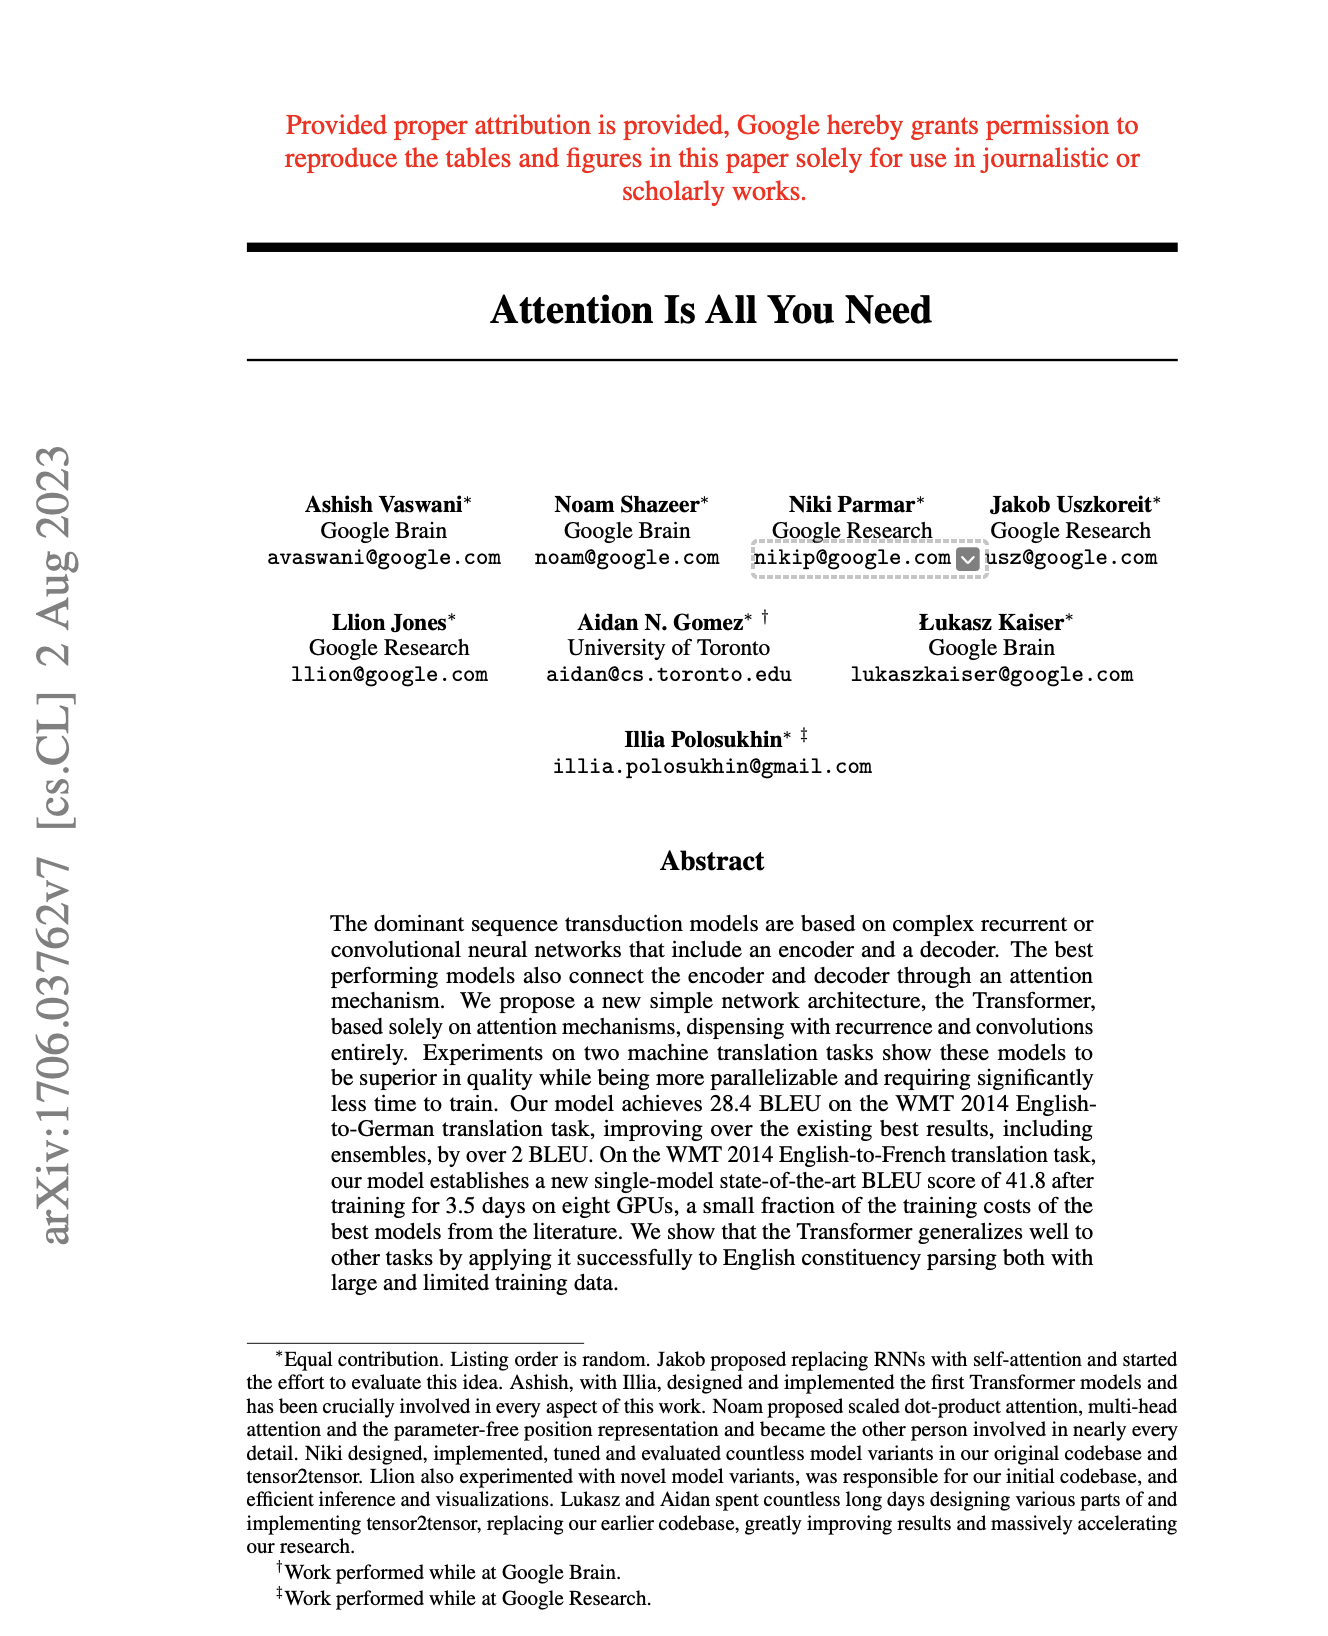
\includegraphics[width=0.8\textwidth]{attentionIsAllYouNeed.png}
\end{minipage}

\end{frame}


\begin{frame}{Transformer Architecture Overview}
  \begin{itemize}
    \item Key innovation: \textbf{self-attention} mechanism allows each token to attend to all others in the sequence.
    \item Enables parallel processing of tokens, unlike RNNs.
    \item Composed of stacked layers of attention and feed-forward networks, with residual connections and normalization.
  \end{itemize}
\end{frame}




\begin{frame}{Self-Attention: What and Why}
  \begin{columns}[T,onlytextwidth]
    \begin{column}{0.6\linewidth}
      \begin{itemize}
        \item \textbf{What}: Each token forms \emph{queries}, \emph{keys}, and \emph{values}: $Q = HW_Q$, $K = HW_K$, $V = HW_V$.
        \item \textbf{Computation}: 
          \[ \text{Attention}(Q,K,V) = \text{softmax}\left(\frac{QK^T}{\sqrt{d_k}}\right)V. \]
        \item \textbf{Why softmax?} Turns similarity scores into a probability distribution to weight values.
        \item \textbf{Why scale by $\sqrt{d_k}$?} Prevents saturation of softmax for large $d_k$, stabilizing training.
         \end{itemize}
    \end{column}
    \begin{column}{0.3\linewidth}
      \begin{exampleblock}{Tiny intuition}
        'The cat sat' $\to$ stronger weights to nearby/related tokens (e.g., 'cat' when processing 'sat').
      \end{exampleblock}
    \end{column}
  \end{columns}
\end{frame}

\begin{frame}{The Transformer at a Glance}
  \begin{itemize}
    \item \textbf{Encoder--Decoder (original paper)}: encoder builds contextual representations; decoder attends to both past outputs (self-attention) and encoder outputs (cross-attention).
    \item \textbf{Encoder-only (BERT family) - representation models}: uses only bidirectional self-attention; effective for understanding tasks.
    \item \textbf{Decoder-only (GPT family) - generative models}: uses only causal/masked self-attention with a mask to prevent peeking ahead; simpler and efficient for generation.
    \item Common building blocks across both: embeddings + positional info, scaled dot-product attention, multi-head projections, residual connections, layer normalization, feed-forward networks.
  \end{itemize}
\end{frame}

\begin{frame}{Neural Machine Translation with Encoder-Decoder RNN}
  \centering
  \begin{tikzpicture}[
    box/.style={rectangle, draw, rounded corners=2pt, minimum height=0.8cm, minimum width=1.5cm, align=center, font=\small},
    inputbox/.style={box, fill=blue!10},
    outputbox/.style={box, fill=green!10},
    encoderbox/.style={rectangle, draw, minimum height=1.2cm, minimum width=8cm, align=center, font=\small, fill=cyan!20},
    decoderbox/.style={rectangle, draw, minimum height=1.2cm, minimum width=8cm, align=center, font=\small, fill=pink!20},
    label/.style={font=\small, align=left, text width=2cm}
  ]

    % Input sequence
    \node[inputbox] (i1) at (1,3.5) {I};
    \node[inputbox] (i2) at (3,3.5) {love};
    \node[inputbox] (i3) at (5,3.5) {robots};

   

    % Encoder
    \node[encoderbox, fill=AMU_acc5!80] (enc) at (3,1.5) {
      \textbf{Encoder (RNN)}\\
      \small Task: representing language
    };
  
    % Decoder
    \node[decoderbox,  fill=AMU_acc6!60] (dec) at (3,-0.5) {
      \textbf{Decoder (RNN)}\\
      \small Task: generating language
    };
   

    % Arrows from encoder to decoder
    \draw[dotted] (enc.south west) -- (dec.north west);
    \draw[dotted] (enc.south east) -- (dec.north east);
    \draw[<->] (enc.south) -- (dec.north) node[midway, right] {}; % Context connection

    % Output sequence
    \node[outputbox] (o1) at (1,-2.5) {Ich};
    \node[outputbox] (o2) at (3,-2.5) {liebe};
    \node[outputbox] (o3) at (5,-2.5) {Roboter};

 % Arrows from input to encoder
    \draw[->] (i1) -- (enc);
    \draw[->] (i2) -- (enc);
    \draw[->] (i3) -- (enc);

    % Arrows from decoder to output
    \draw[->] (dec) -- (o1);
    \draw[->] (dec) -- (o2);
    \draw[->] (dec) -- (o3);

    % Labels
    \node[label, left=0.5cm of i1.west] {Input\\sequence};
    \node[label, left=0.5cm of o1.west] {Output\\sequence};

    % Neural Machine Translation label
    \node[rotate=90, label, anchor=south] at (-1.5,1) {Neural\\machine\\translation};

    % Dotted border around encoder-decoder
    \draw[dotted] ([xshift=-0.5cm,yshift=0.5cm]enc.north west) rectangle ([xshift=0.5cm,yshift=-0.5cm]dec.south east);

  \end{tikzpicture}
\end{frame}

\begin{frame}{LLM Model Timeline (2000--2024)}
  \centering
  \colorlet{colDec}{AMU_acc1!30}
  \colorlet{colEnc}{AMU_acc5!85}
  \colorlet{colED}{AMU_lt2!95}
  \colorlet{colNon}{AMU_acc4!85}

  \begin{tikzpicture}[>=Stealth, thick]
    \tikzset{event/.style={draw=AMU_dk1, rounded corners=2pt, inner xsep=4pt, inner ysep=2pt, font=\footnotesize, align=center}}

    % Baseline: dotted before 2017, solid afterwards
    \draw[dotted, AMU_dk2!95!AMU_lt1] (0,0) -- (2.6,0);
    \draw[->, AMU_acc1] (2.6,0) -- (10,0);

    % Ticks and labels
    \foreach \x/\label in {
      0/{$\sim$2000},
      2.6/2013,
      3.8/2017,
      4.6/2018,
      5.4/2019,
      6.2/2020,
      7.0/2021,
      7.8/2022,
      8.6/2023,
      9.4/2024
    }{
      \draw (\x,0) -- (\x,0.18);
      \node[below=2pt, font=\scriptsize] at (\x,0) {\label};
    }

    % Events
    % Non-transformer
    \draw (0,0) -- (0,0.9);
    \node[event, fill=colNon, anchor=south] at (0,0.9) {Bag-of-words};

    \draw (2.6,0) -- (2.6,1.2);
    \node[event, fill=colNon, anchor=south] at (2.6,1.2) {word2vec};

    \draw (3.8,0) -- (3.8,+0.9);
    \node[event, fill=colNon, anchor=north] at (3.8,+0.9) {Attention};

    % Encoder-only
    \draw (4.5,0) -- (4.5,1.1);
    \node[event, fill=colEnc, anchor=south] at (4.5,1.1) {BERT};

    \draw (5.5,0) -- (5.5,2.25);
    \node[event, fill=colEnc, anchor=south] at (5.5,2.25) {DistilBERT};


    \draw (5.3,0) -- (5.3,1.7);
    \node[event, fill=colEnc, anchor=south] at (5.3,1.7) {RoBERTa};

    
    % Decoder-only
    \draw (4.8,0) -- (4.8,-1.3);
    \node[event, fill=colDec, anchor=north] at (4.8,-1.3) {GPT};

    \draw (5.4,0) -- (5.4,-1.1);
    \node[event, fill=colDec, anchor=south] at (5.4,-1.1) {GPT-2};

    \draw (6.2,0) -- (6.2,-1.8);
    \node[event, fill=colDec, anchor=south] at (6.2,-1.8) {GPT-3};

    \draw (8.4,0) -- (8.4,1.6);
    \node[event, fill=colDec, anchor=south] at (8.4,1.6) {ChatGPT};

    \draw (8.9,0) -- (8.9,1.0);
    \node[event, fill=colDec, anchor=south] at (8.9,1.0) {GPT-4};

    % Encoder-decoder
    \draw (6.4,0) -- (6.4,1.0);
    \node[event, fill=colED, anchor=north] at (6.4,1.0) {T5};

    \draw (7.0,0) -- (7.0,1.0);
    \node[event, fill=colED, anchor=south] at (7.0,1.0) {Switch};

    \draw (8.3,0) -- (8.3,-0.8);
    \node[event, fill=colED, anchor=north] at (8.3,-0.8) {Flan-T5};

    % Legend
    \begin{scope}[shift={(0,-2.2)}]
      \node[event, fill=colDec] at (1.6,0) {\scriptsize Decoder-only};
      \node[event, fill=colEnc] at (4.8,0) {\scriptsize Encoder-only};
      \node[event, fill=colED] at (8.0,0) {\scriptsize Encoder--decoder};
      \node[event, fill=colNon] at (11.2,0) {\scriptsize Non-transformer models};
    \end{scope}
  \end{tikzpicture}
\end{frame}

\begin{frame}{Further Reading on Transformers}
  \begin{itemize}
    \item Highly recommended: \href{https://jalammar.github.io/illustrated-transformer/}{The Illustrated Transformer (Jay Alammar)} for step-by-step visuals.
    \item Optional deeper dive: \href{https://www.deeplearning.ai/short-courses/attention-in-transformers-concepts-and-code-in-pytorch/}{Attention in Transformers (Josh Starmer)} for basic understanding of attention.
    \item Explore attention live: \href{https://poloclub.github.io/transformer-explainer/}{poloclub.github.io/transformer-explainer}

  \end{itemize}
\end{frame}


\begin{frame}{Inference and Decoding Strategies}
  \begin{itemize}
    \item Generation proceeds token by token; decoding choices shape behavior.
    \item \textbf{Temperature}: scales logits to control randomness.
    \item \textbf{Top-$k$} and \textbf{top-$p$ (nucleus)} sampling: restrict candidate tokens to most probable set.
    \item \textbf{Max tokens}: upper bound on generated length; context window includes prompt + output.
    \item Engineering considerations: caching key/value tensors, speculative decoding, batching requests.
  \end{itemize}
\end{frame}

\section{Capabilities and Limitations}

\begin{frame}{What LLMs Do Well}
  \begin{itemize}
    \item Few-shot learning: adapt to new tasks using examples in the prompt.
    \item Chain-of-thought prompting: articulate intermediate reasoning steps.
    \item Code generation and refactoring for Python, SQL, and beyond.
    \item Summarization, translation, explanation across domains.
    \item Data-wrangling assistance: regex creation, feature brainstorming, doc parsing.
  \end{itemize}
\end{frame}

\begin{frame}{Limits, Risks, Practices}
  \begin{itemize}
    \item \textbf{Hallucinations}: confident but fabricated answers without grounding.
    \item \textbf{Inconsistency}: outputs vary with phrasing, temperature, and randomness.
    %\item \textbf{Lack of true reasoning}: pattern matching, not deep understanding
    \item \textbf{Context window limits}: finite memory (e.g., 8k--200k tokens) affects long documents.
    \item \textbf{Bias and toxicity}: inherited from training data, requiring audits and guardrails.
    \item \textbf{Cost and latency}: API tokens and GPU serving are not free; optimize prompts and batching.
    \item \textbf{No persistent memory}: model forgets state across sessions unless you build storage.
    \item \textbf{Data privacy}: be cautious with sensitive info; follow provider policies.
    \item \textbf{Best practices}: clear prompts, few-shot examples, temperature tuning, output validation.
    \item \textbf{Human-in-the-loop}: always review critical outputs; LLMs assist, not replace, human judgment.
  \end{itemize}
\end{frame}

\section{Ecosystem and Access}

% =========================
% Slide 1 — Hosted APIs
% =========================
\begin{frame}{Where to Get Models (Hosted APIs)}
  \vspace{-0.3em}
  \textbf{Major providers (managed, pay-per-use; fast start)}
  \begin{center}
    \begin{tabular}{@{}lll@{}}
      \toprule
      Provider & Example Models (2025) & Access \\
      \midrule
      OpenAI & o4-mini, o3, GPT-4o & Hosted API (reasoning, vision) \\
      Google DeepMind & Gemini 2.5 Pro / Flash & Gemini API (free tier + paid) \\
      Anthropic & Claude Sonnet 4.5 & Claude API / Console \\
      xAI & Grok-4, Grok-3 & API (OpenAI-compatible) \\
      % (Optional) Cohere & Command R+ & Hosted API (RAG/tool use) \\
      \bottomrule
    \end{tabular}
  \end{center}

  \vspace{0.6em}
  \textbf{When to choose}
  \begin{itemize}
    \item Minimal ops, latest frontier models, strong tooling \& SLAs.
    \item Cons: recurring cost, data governance/contracts, rate limits.
  \end{itemize}
\end{frame}

% =========================
% Slide 2 — Open Weights & Hubs
% =========================
\begin{frame}{Where to Get Models (Open Weights \& Hubs)}
  \vspace{-0.3em}
  \textbf{Open models (self-host or use hosted endpoints)}
  \begin{center}
    \begin{tabular}{@{}lll@{}}
      \toprule
      Provider & Example Models (2025) & Access \\
      \midrule
      Meta & Llama 3.1, Llama 4 (Scout/Maverick) & Open weights (license) \\
      Mistral & Mistral Large/Medium/Small, Pixtral & Open weights \& Mistral API \\
      Microsoft & Phi-4, Phi-4-reasoning & Open weights (HF) \\
      Hugging Face Hub & Falcon, Mixtral, Phi, etc. & Hub + Inference API/Endpoints \\
      \bottomrule
    \end{tabular}
  \end{center}

  \vspace{0.6em}
  \textbf{When to choose}
  \begin{itemize}
    \item Control, on-prem/privacy, cost efficiency at scale.
    \item Cons: you manage serving, scaling, evals, safety layers.
  \end{itemize}
\end{frame}

\begin{frame}[fragile]{Calling an API}
  \begin{lstlisting}[language=Python]
from openai import OpenAI
client = OpenAI()

resp = client.chat.completions.create(
    model="gpt-4o-mini",
    messages=[
        {"role": "system", "content": "You are a data assistant."},
        {"role": "user", "content": "Tell me a joke about matrix inversion."}
    ],
    temperature=0.6,
    max_tokens=120,
)
print(resp.choices[0].message.content)
  \end{lstlisting}
\end{frame}


\section{Wrap-Up}

\begin{frame}{Further Reading}
  \vspace{-0.4em}
  \begin{tabular}{@{}p{3.8cm}p{7.8cm}@{}}
    \toprule
    \textbf{Concept} & \textbf{Reference / Why it matters} \\
    \midrule
    LLM overview & \href{https://learn.deeplearning.ai/courses/how-transformer-llms-work}{How Transformer LLMs Work (deeplearning.ai)} — concise intro to components. \\
    Transformer basics & \href{https://jalammar.github.io/illustrated-transformer/}{The Illustrated Transformer (Jay Alammar)} — visual intuition for attention. \\
    %Tokenization & \href{https://github.com/openai/tiktoken}{OpenAI \texttt{tiktoken}}; \href{https://huggingface.co/docs/tokenizers/index}{HF Tokenizers} — counts, costs, subwords. \\
    Attention math & \href{https://arxiv.org/abs/1706.03762}{Attention Is All You Need (Vaswani et al., 2017)} — original paper. \\
    %Scaling laws & \href{https://arxiv.org/abs/2005.14165}{GPT-3 (Brown et al., 2020)}; \href{https://arxiv.org/abs/2203.15556}{Chinchilla (Hoffmann et al., 2022)} — compute/data trade-offs. \\
    APIs (OpenAI) & \href{https://platform.openai.com/docs}{OpenAI Platform Docs} — endpoints, auth, safety. \\
    APIs (Gemini) & \href{https://ai.google.dev/gemini-api/docs}{Gemini API Docs} — free tier + multimodal. \\
    APIs (Claude) & \href{https://docs.anthropic.com}{Anthropic Claude Docs} — reasoning, tool use. \\
    APIs (Grok) & \href{https://x.ai/api}{xAI Grok API} — OpenAI-compatible endpoints. \\
     \bottomrule
  \end{tabular}
\end{frame}
\end{document}
